\documentclass[acmsmall,screen,review,anonymous]{acmart}

\usepackage{booktabs}
\usepackage{tabularx}
\usepackage{array}
\usepackage{url}

\emergencystretch=1em
\raggedbottom

\setcopyright{none}
\settopmatter{printacmref=false}
\renewcommand\footnotetextcopyrightpermission[1]{}
\acmJournal{TIST}
\acmYear{2027}
\acmVolume{0}
\acmNumber{0}
\acmArticle{0}
\acmMonth{1}

\begin{document}

\title[Presentation Priors in Language Models]{Presentation Priors in Language Models: Default Formatting, Instruction Spillover, and Their Emergence in Post-Training}

\author{Anonymous Authors}
\affiliation{%
  \institution{Anonymous Institution}
  \country{Anonymous}
}

\begin{abstract}
When a prompt leaves presentation unspecified, a language model still has to choose it: whether to use emoji, Markdown, lists, or a particular color. We call the resulting regularities \emph{presentation priors} and measure them in five studies. Emoji defaults are topic-conditioned: without instructions, 94--98\% of social-media outputs from each of three models contain emoji, while legal and technical outputs contain none. In unrestricted color suggestions, three models converge on a few conventional blues. A controlled probe of six models, including three frontier models, across 60 prompts and eight conditions finds Markdown in 46--100\% of neutral outputs; an enumerated plain-prose instruction reduces it to at most 4.4\%, and it works the same whether placed in the system or the user prompt. An instruction-matched placebo that names no presentation feature removes emoji in all four models that use emoji and removes most Markdown in three models, so intervention effects mix what an instruction says with the effect of adding an instruction. Finally, across the openly released training stages of one 1B model, Markdown rises from 13\% of outputs after supervised fine-tuning to 50\% after preference optimization, with a five-fold increase in Markdown density; the ability to suppress Markdown on request appears at the same stage. We report prompt-clustered uncertainty, model-route censoring, and detector limits.
\end{abstract}

\keywords{language models, instruction following, output format bias, presentation priors, homogenization, model evaluation}

\maketitle

\section{Introduction}

Short prompts now produce messages, notices, and product copy that people paste directly into other systems. Such prompts rarely say how the output should look. A request for a launch note does not say whether to use emoji, headings, bullet points, or exclamation marks; a request for a brand palette does not say which hue to start from. The model fills these gaps, and what it fills them with is a property of the model rather than of the request.

This article treats those choices as an evaluation target. We use \emph{presentation priors} for measurable surface-form regularities that appear when a prompt leaves presentation open, and we measure them together with the interventions that suppress them. Presentation priors are not necessarily failures. A Markdown list can be the most useful answer, and a provider may document a formatting default on purpose. Our interest is in what the model chooses when nobody asked, how strongly that choice depends on topic and model, and how it responds to instructions.

Three results go beyond the expected finding that explicit formatting instructions are usually obeyed. The first is \emph{instruction spillover}. Interventions change features they do not mention: an instruction-matched placebo that forbids no presentation feature removes emoji from every model that uses emoji, and an emoji-only prohibition removes most Markdown. Condition-versus-neutral contrasts therefore conflate a content-specific effect with a generic effect of adding an instruction. The second is \emph{where the Markdown default emerges}. Across the released training stages of one open model, the default appears at the preference-optimization step, together with the ability to switch it off. The third is \emph{palette convergence}: in an unrestricted color-suggestion task, three models concentrate on a small set of blue primaries, several of which are the primary colors of widely used design systems.

We make five contributions:
\begin{itemize}
  \item We define presentation priors, the prior-plus-override curve, and instruction spillover as separate measurement targets, distinct from semantic instruction following.
  \item We re-analyze three earlier text studies per model with prompt-clustered uncertainty, disclose where model-route failures censor the data, and replace an earlier color result with a palette-convergence analysis (Sections~\ref{sec:study1}--\ref{sec:study3}).
  \item We run a controlled probe of six models across 60 prompts and eight conditions, including an instruction-matched placebo, a single-prohibition condition, and system-prompt placement (Section~\ref{sec:study4}).
  \item We trace Markdown and emoji defaults across the base, supervised fine-tuning, preference-optimization, and final checkpoints of one open model (Section~\ref{sec:study5}).
  \item We quantify instruction spillover and argue that intervention studies of model formatting need instruction-matched controls (Section~\ref{sec:spillover}).
\end{itemize}

Our claims are bounded. The training-stage evidence comes from a single 1B model family, and its base checkpoint is prompted without a chat template, so it shows where the default emerges in that family rather than a general mechanism. We report no human-perception data, and our detectors are transparent heuristics whose limits we document in Section~\ref{sec:validity}.

\section{Definitions}

\paragraph{Presentation prior.} A measurable surface-form regularity that appears when a model completes a task whose presentation is unspecified: for example, emoji in short social copy, Markdown in an advisory note, exclamation marks in an announcement, or a blue primary color in a palette. We call it a prior because it appears without being requested, not because it is unintended. Some priors are documented provider defaults; we measure them all the same way.

\paragraph{Prior-plus-override curve.} The rate of a feature under a neutral prompt, followed by its rate under one or more interventions that suppress or redirect it.

\paragraph{Surface-form compliance.} Satisfaction of mechanically checkable presentation constraints such as ``no emoji'' or ``under 150 words''. We keep it separate from semantic instruction following, factuality, and task success.

\paragraph{Instruction spillover.} A change in a feature that an intervention does not mention, such as a drop in Markdown after an emoji-only prohibition. A condition-versus-neutral contrast estimates the sum of the content-specific effect and the spillover; a control condition is needed to separate them.

\section{Related Work}
\label{sec:related}

\paragraph{Format and style bias in alignment and evaluation.} Preference models and LLM judges reward particular presentation. Zhang et al.\ show that human raters, GPT-4, and reward models prefer lists, links, bold text, and emoji, and that models can exploit these preferences to rank higher on AlpacaEval and Chatbot Arena \cite{zhang2025lists}. Chatbot Arena \cite{chiang2024chatbot} now reports style-controlled rankings that treat length and Markdown as covariates \cite{li2024style}, and LLM judges favour style over substance \cite{feuer2025style} and longer answers \cite{zheng2023judging,saito2023verbosity}. Length is the best-studied case: much of the reward gain in RLHF can come from length alone \cite{singhal2024length}, length-controlled evaluation reduces judge bias \cite{dubois2024length}, and direct preference optimization exploits length in preference data \cite{park2024disentangling}. These works explain why presentation features may be rewarded during post-training \cite{ouyang2022training,rafailov2023direct}. We measure the resulting behavior at generation time, when the user specifies nothing, and how instructions move it.

\paragraph{Superficial alignment.} Alignment changes mostly stylistic behavior. LIMA reaches strong performance after fine-tuning on 1,000 curated examples, suggesting that alignment mainly teaches response style and format \cite{zhou2023lima}, and base and aligned models differ mostly on stylistic tokens \cite{lin2024unlocking}. RLHF also reduces output diversity relative to supervised fine-tuning \cite{kirk2024understanding}. Presentation priors are a measurable trace of this stylistic layer. Openly released stage-wise models such as T\"ulu 3 \cite{lambert2024tulu} and OLMo 2 \cite{olmo2025furious} make it possible to locate where a prior emerges; Study 5 uses the OLMo 2 checkpoints for this purpose.

\paragraph{Instruction following and format constraints.} IFEval \cite{zhou2023ifeval} and FollowBench \cite{jiang2024followbench} measure whether stated, verifiable constraints are satisfied, and accuracy falls as the number of simultaneous instructions grows \cite{harada2025instructions}. Format matters in other ways too: models are biased toward particular output formats \cite{long2025format}, format restrictions such as JSON degrade reasoning \cite{tam2024speak}, and meaning-preserving changes to prompt formatting shift accuracy substantially \cite{sclar2024quantifying}. Instruction hierarchies govern how system and user instructions interact \cite{wallace2024instruction}. These benchmarks score compliance with stated requirements. We also measure what appears when nothing is stated, and we show that interventions change features they do not mention, which compliance scores alone cannot reveal.

\paragraph{Model idiosyncrasies and LLM style.} Outputs of different LLMs are separable: a text-embedding classifier identifies which of five models wrote a text with 97\% accuracy \cite{sun2025idiosyncrasies}. Corpus-level studies track LLM style through word-frequency shifts in peer reviews \cite{liang2024monitoring} and biomedical abstracts \cite{kobak2025delving}. Our features are coarser and fully transparent, and we study them as defaults under controlled prompts rather than as identifiers.

\paragraph{Homogenization.} Writing with an instruction-tuned model reduces content diversity across authors \cite{padmakumar2024writing}, AI-assisted stories are more similar to each other \cite{doshi2024generative}, and ChatGPT users produce less distinct ideas \cite{anderson2024homogenization}. More broadly, shared models can homogenize outcomes \cite{bommasani2022picking}. Text-diversity metrics such as distinct-$n$ \cite{li2016diversity} measure lexical variety. The palette convergence in Study 2 is a presentation-level instance of homogenization.

\paragraph{Generative interfaces and images.} Models increasingly generate UI code and interface actions \cite{wu2024uicoder,kong2026macaron}, and text-to-image work documents representational bias \cite{bianchi2022t2i,friedrich2024fairness}. Corpora of human-designed interfaces \cite{deka2017rico,wu2023webui} could supply the reference distributions that studies of cross-modal defaults need. We leave cross-modal analysis to companion work.

\section{Relation to Earlier Versions}
\label{sec:prior-versions}

Studies 1--3 use datasets that the authors reported in earlier manuscripts (anonymized for review; details provided to the editors). Those manuscripts pooled results across models and framed them as instruction-following or security findings. Table~\ref{tab:delta} lists what is new here. Studies 4 and 5 are entirely new; Study 4 replaces a smaller first-pass probe (480 outputs, four routes, one prompt per family) whose tables appear in Appendix~\ref{app:pilot}. The cross-modal UI and image analyses of earlier versions are not part of this article.

\begin{table}[t]
\centering
\caption{What this article adds to the earlier versions of each study.}
\label{tab:delta}
\begin{tabularx}{\linewidth}{>{\raggedright\arraybackslash}p{0.17\linewidth}>{\raggedright\arraybackslash}p{0.25\linewidth}>{\raggedright\arraybackslash}X}
\toprule
Study & Status in earlier versions & New in this article \\
\midrule
1: Emoji defaults & Pooled compliance by instruction level & Per-model curves with prompt-clustered intervals; censoring analysis; detector sensitivity; genre caveat \\
2: Color suggestions & Pooled purple and gradient counts & Restricted to the unrestricted variant; palette-convergence analysis; gradient claim withdrawn as a compliance measure \\
3: Multiple constraints & Pooled violation counts & Per-model table; coverage disclosure; surface-versus-semantic claim withdrawn \\
4: Controlled probe & First-pass pilot only & Entire study: 60 prompts, six models, placebo and system-prompt conditions \\
5: Training stages & Not reported & Entire study \\
\bottomrule
\end{tabularx}
\end{table}

\section{Data and Common Method}
\label{sec:method}

Table~\ref{tab:data} summarizes the collections. In the artifact, Studies 1--3 are Experiments 1, 2, and 4; Studies 4 and 5 are the hosted and local parts of Experiment 8 v2, and the pilot is Experiment 8 v1; the remaining experiment numbers belong to unrelated studies. Hosted models were queried through API routes at fixed sampling settings; only the system-prompt condition of Study 4 uses a system prompt. Route identifiers are recorded in the artifact. The GPT-3.5-Turbo route was queried in early 2026 under the identifier \texttt{gpt-3.5-turbo-0613}; we could not verify which upstream snapshot served it.

\begin{table}[t]
\centering
\caption{Collections analyzed. Temperature was fixed within each collection. ``Clean'' excludes API failures.}
\label{tab:data}
\begin{tabularx}{\linewidth}{>{\raggedright\arraybackslash}p{0.12\linewidth}>{\raggedright\arraybackslash}p{0.28\linewidth}>{\raggedright\arraybackslash}X r r}
\toprule
Study & Models (collection month) & Design & Clean / total & Temp. \\
\midrule
1 & Gemini 2.5 Flash, GPT-3.5-Turbo, GLM-4.5 Air (Feb 2026) & 6 topics $\times$ 4 prompts $\times$ 5 instruction levels $\times$ 30 runs & 9,658 / 10,800 & 0.7 \\
2 & Gemini 2.5 Flash, GPT-3.5-Turbo, MiMo v2 Flash (Mar--Apr 2026) & 5 company types $\times$ 3 variants $\times$ 30 runs; 450 unrestricted rows analyzed & 1,350 / 1,350 & 0.7 \\
3 & Gemini 2.5 Flash, GPT-3.5-Turbo, GLM-4.5 Air (Mar 2026) & 5 topics $\times$ 8 constraint sets $\times$ 30 runs & 2,504 / 3,600 & 0.7 \\
4 & Claude Sonnet 5.5, Claude Haiku 5.5, Gemini 3.8 Flash, Qwen 3.6 Flash, Llama 3.3 70B and 3.1 8B Instruct (Nov 2026) & 12 families $\times$ 5 prompts $\times$ 8 conditions $\times$ 3 repeats, randomized order & 8,640 / 8,640 & 0.8 \\
5 & OLMo 2 1B: base, SFT, DPO, instruct checkpoints, run locally (Nov 2026) & 60 prompts $\times$ 7 conditions $\times$ 1 run & 1,680 / 1,680 & 0.8 \\
Pilot & Llama 3.3 70B, Llama 3.1 8B, Qwen 2.5 7B (Instruct), Qwen 3.6 Flash (Jun 2026) & 12 prompt families $\times$ 5 conditions $\times$ 2 repeats & 480 / 480 & 0.8 \\
\bottomrule
\end{tabularx}
\end{table}

\paragraph{Detectors.} Features are computed from output text with transparent rules: emoji and decorative symbols by Unicode ranges; Markdown by headings, list markers, emphasis, inline code, and links; polish by exclamation marks or a ten-word stock-phrase lexicon; and colors by hexadecimal codes converted to HSL. The \texttt{format\_default} composite fires on emoji, Markdown, or decorative symbols. Section~\ref{sec:validity} documents known weaknesses of each detector.

\paragraph{Uncertainty.} Repeated samples of the same prompt are not independent, so we never treat outputs as the unit of inference. For Studies 1--3 we report intervals from a prompt-cluster bootstrap (2,000 resamples of whole prompts). For Studies 4 and 5, inferential statements use paired differences between conditions (or stages) computed within each of the 60 prompts, with repeats averaged within prompt, a sign-flip test over prompts, and prompt-cluster bootstrap intervals. Models are treated as fixed, so results describe these models and do not generalize to a population of models.

\paragraph{Missing data.} Studies 1 and 3 include a free GLM route that failed with rate-limit and connection errors. Failures are not random with respect to condition, because collection ran in blocks by condition. We therefore report every result per model and state which cells are censored. In Study 4, Qwen 3.6 Flash returned an empty response for 181 tasks because hidden reasoning consumed the 1,500-token budget; the empty responses concentrated in the placebo (83) and diversity (56) conditions. One retry at the same budget recovered 94 of them, and the remaining 87 were retried at 6,000 tokens, so Study 4 has no missing outputs.

\section{Study 1: Topic-Conditioned Emoji Defaults}
\label{sec:study1}

Study 1 asks models to write on six topic families under five instruction levels, from no instruction (L0) through a polite request (L1) to emphatic and contextual prohibitions (L3--L4). Table~\ref{tab:study1-model-level} reports the emoji-free rate per model.

\begin{table}[t]
\centering

\caption{E1: emoji-free rate by model and instruction level, with 95\% intervals from a prompt-cluster bootstrap. Missing rows are HTTP 429 rate-limit failures on the free GLM route; GLM has no L4 rows and its L3 rows cover only academic, legal, and technical prompts.}
\label{tab:study1-model-level}
\begin{tabular}{llrrr}
\toprule
Model & Level & Clean & Missing & Emoji-free \% [95\% CI] \\
\midrule
Gemini 2.5 Flash & L0 & 720 & 0 & 81.7 [65.8, 95.0] \\
 & L1 & 720 & 0 & 100.0 [100.0, 100.0] \\
 & L2 & 720 & 0 & 100.0 [100.0, 100.0] \\
 & L3 & 720 & 0 & 100.0 [100.0, 100.0] \\
 & L4 & 720 & 0 & 100.0 [100.0, 100.0] \\
GPT-3.5-Turbo & L0 & 720 & 0 & 82.1 [66.5, 95.8] \\
 & L1 & 720 & 0 & 100.0 [100.0, 100.0] \\
 & L2 & 720 & 0 & 100.0 [100.0, 100.0] \\
 & L3 & 720 & 0 & 100.0 [100.0, 100.0] \\
 & L4 & 720 & 0 & 100.0 [100.0, 100.0] \\
GLM-4.5 Air & L0 & 718 & 2 & 68.1 [52.1, 84.1] \\
 & L1 & 701 & 19 & 96.1 [91.2, 99.4] \\
 & L2 & 684 & 36 & 99.1 [97.3, 100.0] \\
 & L3 & 355 & 365 & 100.0 [100.0, 100.0] \\
 & L4 & 0 & 720 & -- \\
\bottomrule
\end{tabular}
\end{table}


Without instructions, emoji use is sharply topic-conditioned in every model. Social-media prompts produce emoji in 97.5\% (Gemini), 96.7\% (GPT-3.5), and 94.2\% (GLM) of outputs, while legal and technical prompts produce none in any model. Three of the four social-media prompts name genres in which emoji are conventional (an Instagram caption, a tweet thread, and a LinkedIn post), so the social-media rate measures adherence to genre convention as much as an unprompted preference. The prompt-cluster intervals at L0 are wide (for example, 65.8--95.0\% emoji-free for Gemini) because emoji use varies strongly across prompts within a topic.

The override is a step, not a curve. Gemini and GPT-3.5 are emoji-free in all 720 outputs at every level from L1 onward. GLM is 96.1\% emoji-free at L1 and 99.1\% at L2; all 27 non-compliant L1 outputs are marketing or social-media outputs. Stronger levels cannot be assessed for GLM: its free route failed with HTTP 429 rate-limit errors on all 720 L4 attempts and on 365 of 720 L3 attempts, leaving no L3 data for the marketing, recipe, or social-media topics. The earlier versions' pooled ``100\% at L3--L4'' result therefore reflects a change in model mix, and we no longer report it.

Detector sensitivity: 14 of the 523 non-compliant outputs (all GLM, at L1 or L2) contain only check marks or geometric symbols that the emoji pattern matches but that are not pictographic emoji. Reclassifying them does not change any conclusion.

\section{Study 2: Palette Convergence in Color Suggestions}
\label{sec:study2}

Study 2 asks for a primary, secondary, and accent color for five company types. Two of its three variants explicitly forbid purple, pink, and gradients, so they measure compliance rather than defaults. We analyze only the 450 unrestricted responses, in which the prompt requests three hexadecimal colors and nothing else (Table~\ref{tab:study2-palette}, Figure~\ref{fig:study2-palette}).

\begin{table}[t]
\centering
\small
\caption{E2: primary colors in the unrestricted baseline variant (150 responses per model, 5 company types). Blue: saturated-blue primaries, defined as hue 190--260$^\circ$, saturation $\geq$30\%, lightness 20--90\%.}
\label{tab:study2-palette}
\begin{tabular}{lrrlr}
\toprule
Model & Blue & Distinct & Top-3 primaries (count) & Purple \\
\midrule
Gemini 2.5 Flash & 85/150 & 24 & \texttt{2C3E50} (46), \texttt{007BFF} (44), \texttt{004D40} (8) & 0 \\
GPT-3.5-Turbo & 133/150 & 26 & \texttt{1A73E8} (39), \texttt{004B8D} (17), \texttt{2C3E50} (13) & 0 \\
MiMo v2 Flash & 102/150 & 34 & \texttt{2563EB} (33), \texttt{0A2540} (17), \texttt{005B96} (15) & 1 \\
\bottomrule
\end{tabular}
\end{table}


\begin{figure}[t]
\centering
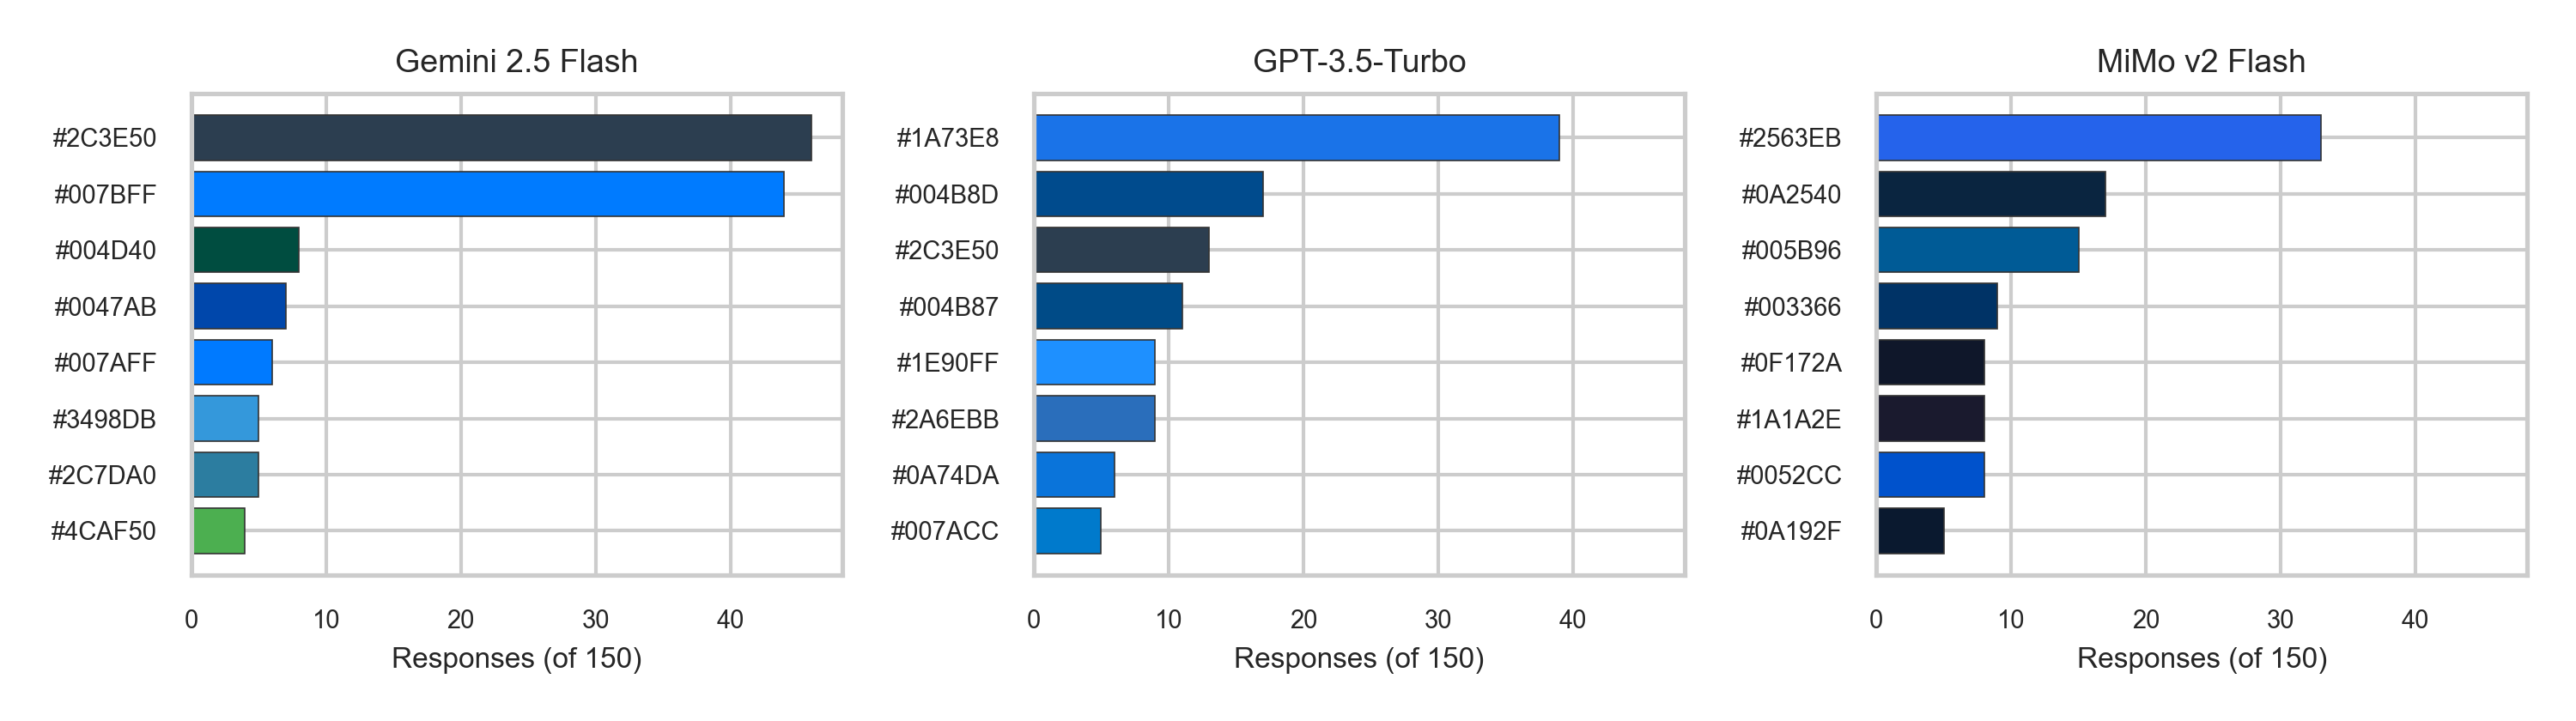
\includegraphics[width=\linewidth]{../analysis_output/tist_revision/figures/study2_primary_colors.png}
\caption{The eight most frequent primary colors per model in the unrestricted variant of Study 2 (150 responses per model). Bars are drawn in the color they count.}
\label{fig:study2-palette}
\end{figure}

The primaries converge. Saturated blue is the primary in 133 of 150 GPT-3.5 responses, 102 of 150 MiMo responses, and 85 of 150 Gemini responses. The most common Gemini primary, \texttt{\#2C3E50}, is a dark desaturated slate that our saturation threshold excludes, so Gemini's blue share is a conservative count. Each model uses only 24--34 distinct primaries across 150 responses and five unrelated sectors, and its three most frequent primaries account for 43--65\% of its responses. Several of the most frequent values are the primary colors of widely used design systems: \texttt{\#007BFF} is Bootstrap's primary blue, \texttt{\#1A73E8} is Google's product blue, and \texttt{\#2563EB} is Tailwind's \texttt{blue-600}. Purple or pink appears in 1 of the 450 unrestricted responses.

We draw two conclusions. The data do not support a broad preference for purple in this task. The stronger finding is convergence: the models largely reproduce a few conventional blues, so they may be echoing common human design-system defaults rather than inventing new ones. Without a reference distribution of human-designed palettes we cannot say whether the models are more concentrated than designers are; Section~\ref{sec:validity} discusses this baseline. Earlier versions also reported gradient use. The unrestricted variant's template cannot express a gradient, and the only CSS variant explicitly forbids gradients, so the two CSS gradients we observe (both from MiMo, in that variant) are compliance failures and say nothing about a gradient default.

\section{Study 3: Surface Constraints Stated Together}
\label{sec:study3}

Study 3 adds surface constraints cumulatively (no emoji, no bullets, no headers, no bold or italic, and a word limit) across five expository topics. Table~\ref{tab:study3-model} reports violations per model.

\begin{table}[t]
\centering

\caption{E3: violations / active rows by model. GLM retains 104 of 1,200 rows after connection errors and has no rows in progressive conditions 4--7; its 28 word-limit rows all come from the full-constraint condition.}
\label{tab:study3-model}
\begin{tabular}{lrrr}
\toprule
Constraint & Gemini 2.5 Flash & GPT-3.5-Turbo & GLM-4.5 Air \\
\midrule
No emoji & 0/1200 & 0/1200 & 0/104 \\
No bullets & 0/1050 & 0/1050 & 0/76 \\
No headers & 0/900 & 0/900 & 0/49 \\
No bold/italic & 3/750 & 0/750 & 0/28 \\
Word limit & 11/300 & 3/300 & 0/28 \\
\bottomrule
\end{tabular}
\end{table}


Violations are rare: 3 bold or italic violations in 750 active Gemini rows, and 11 (Gemini) and 3 (GPT-3.5) word-limit violations in 300 active rows each. Three caveats limit the interpretation. First, GLM contributes only 104 rows after connection errors and none in progressive conditions 4--7, so the study is effectively a two-model study. Second, the no-emoji constraint is active in every condition and there is no unconstrained arm; Study 1 shows that expository topics rarely produce emoji anyway, so perfect emoji compliance here cannot be told apart from the feature never appearing. Third, constraints are added in a fixed order, so the number of constraints is confounded with which constraints are active. Study 3 therefore shows only that these surface constraints are easy to satisfy when stated. Earlier versions also contrasted surface and semantic constraints; Study 3 contains no semantic constraints, so we withdraw that claim.

\section{Study 4: A Controlled Probe of Six Models}
\label{sec:study4}

Study 4 crosses six models, twelve prompt families with five prompts each, and eight conditions, with three repeats per cell and a randomized execution order. Besides the neutral prompt, the conditions append ``Do not use emoji.'' (no-emoji), ``Do not use Markdown formatting.'' (no-Markdown), an enumerated plain-prose instruction (plain), an instruction-matched placebo, a request for domain-specific, non-generic writing (diverse), and a request for polished writing in plain prose; a final condition moves the plain instruction from the user prompt to the system prompt. The placebo matches the plain instruction in length and imperative form but forbids only non-presentational failures: ``Write carefully. Do not leave out the main point, invent facts, contradict yourself, use placeholder text, introduce undefined jargon, or address the wrong audience.'' Table~\ref{tab:v2-routes} reports the main contrasts.

\begin{table}[t]
\centering
\footnotesize
\caption{Study 1 (60 prompts in 12 families, 3 repeats per cell). Neutral rates (\%) for markup syntax (headings, emphasis, code, links, tables), list lines, and emoji. Other columns: change versus neutral in percentage points, computed within prompt and averaged within family; * marks Holm-adjusted $p<0.05$ (exact sign-flip test over the 12 families, 35 tests). NE, No-MD, Plain: markup change under the no-emoji, bare no-Markdown, and enumerated plain-prose instructions; P: mk and P: em: markup and emoji change under the placebo.}
\label{tab:v2-routes}
\begin{tabular}{lrrrrrrrr}
\toprule
Model & Markup & Lists & Emoji & NE & No-MD & Plain & P: mk & P: em \\
\midrule
Claude Sonnet 5.5 & 100.0 & 63.3 & 21.7 & -6.7 & -100.0* & -100.0* & -2.2 & -17.8 \\
Gemini 3.8 Flash & 97.8 & 51.1 & 31.7 & -54.4 & -97.8* & -97.8* & -62.2* & -31.7 \\
Qwen 3.6 Flash & 87.2 & 43.9 & 46.1 & -52.8* & -87.2* & -87.2* & -65.0* & -43.9* \\
Claude Haiku 5.5 & 75.6 & 50.6 & 8.9 & -14.4 & -75.6* & -75.6* & -5.0 & -8.9 \\
Llama 3.1 8B & 68.3 & 58.3 & 0.0 & -52.2* & -47.8* & -68.3* & +0.0 & +0.0 \\
GPT-5.6 Luna & 48.3 & 0.0 & 7.8 & -14.4 & -48.3 & -48.3 & -6.1 & -6.1 \\
Llama 3.3 70B & 38.3 & 31.1 & 0.0 & -38.3 & -38.3 & -38.3 & -32.2 & +0.0 \\
\bottomrule
\end{tabular}
\end{table}


Markdown is the dominant prior. Neutral outputs contain it in 100\% (Claude Sonnet 5.5), 97.8\% (Gemini 3.8 Flash), 87.2\% (Qwen 3.6 Flash), 78.3\% (Claude Haiku 5.5), 73.3\% (Llama 3.1 8B), and 46.1\% (Llama 3.3 70B) of cases. Emoji is a minority prior concentrated in four models: 46.1\% (Qwen), 31.7\% (Gemini), 21.7\% (Sonnet), and 8.9\% (Haiku); neither Llama model produces emoji under any condition.

Stated requirements are obeyed when they are enumerated. The plain instruction leaves Markdown in at most 4.4\% of outputs (Llama 3.1 8B; 0\% for the other five models), and moving it into the system prompt changes nothing: the system-versus-user difference is at most 0.6 percentage points for every model. A bare ``Do not use Markdown formatting'' works less well, leaving Markdown in 38.3\% (Sonnet), 33.9\% (Llama 3.1 8B), and 14.4\% (Haiku) of outputs. Part of this residue reflects a definitional gap: our detector counts numbered and bulleted lines as Markdown, while a model may read ``Markdown formatting'' as headings and emphasis only.

The diverse condition lowers emoji in every model that uses emoji (by 8.9 to 43.3 points) and lowers Markdown for Gemini ($-15.0$) and Qwen ($-28.3$), but not for the Claude or Llama models. Like the placebo results below, this is consistent with a generic effect of adding an instruction.

\section{Study 5: Where the Markdown Default Emerges}
\label{sec:study5}

Study 5 runs the same 60 prompts and seven conditions (all except system placement) on the four released checkpoints of OLMo 2 1B: the pretrained base model, the supervised fine-tuned (SFT) model, the preference-optimized (DPO) model, and the final instruct model trained further with reinforcement learning on verifiable rewards \cite{olmo2025furious,lambert2024tulu}. The three post-trained checkpoints receive the prompt through their chat template; the base checkpoint has no chat template, so it receives the bare instruction and continues the text. Each prompt and condition is generated once per checkpoint on local hardware. Table~\ref{tab:v2-stages} and Figure~\ref{fig:olmo-stages} report the results.

\begin{table}[t]
\centering
\small
\caption{Study 5: OLMo 2 1B checkpoints by training stage (60 prompts, one output each per condition). Rates in \%; MD/100w (Markdown markers per 100 words) and words are neutral-condition means.}
\label{tab:v2-stages}
\begin{tabular}{lrrrrrrrr}
\toprule
Stage & Neutral MD & Emoji & Placebo MD & Emoji & Plain MD & Emoji & MD/100w & Words \\
\midrule
Base & 33.3 & 0.0 & 41.7 & 0.0 & 45.0 & 3.3 & 1.9 & 297 \\
SFT & 13.3 & 1.7 & 10.0 & 1.7 & 21.7 & 5.0 & 0.6 & 75 \\
DPO & 50.0 & 6.7 & 73.3 & 6.7 & 28.3 & 3.3 & 3.2 & 189 \\
Instruct (RLVR) & 53.3 & 6.7 & 75.0 & 8.3 & 10.0 & 0.0 & 2.6 & 168 \\
\bottomrule
\end{tabular}
\end{table}


\begin{figure}[t]
\centering
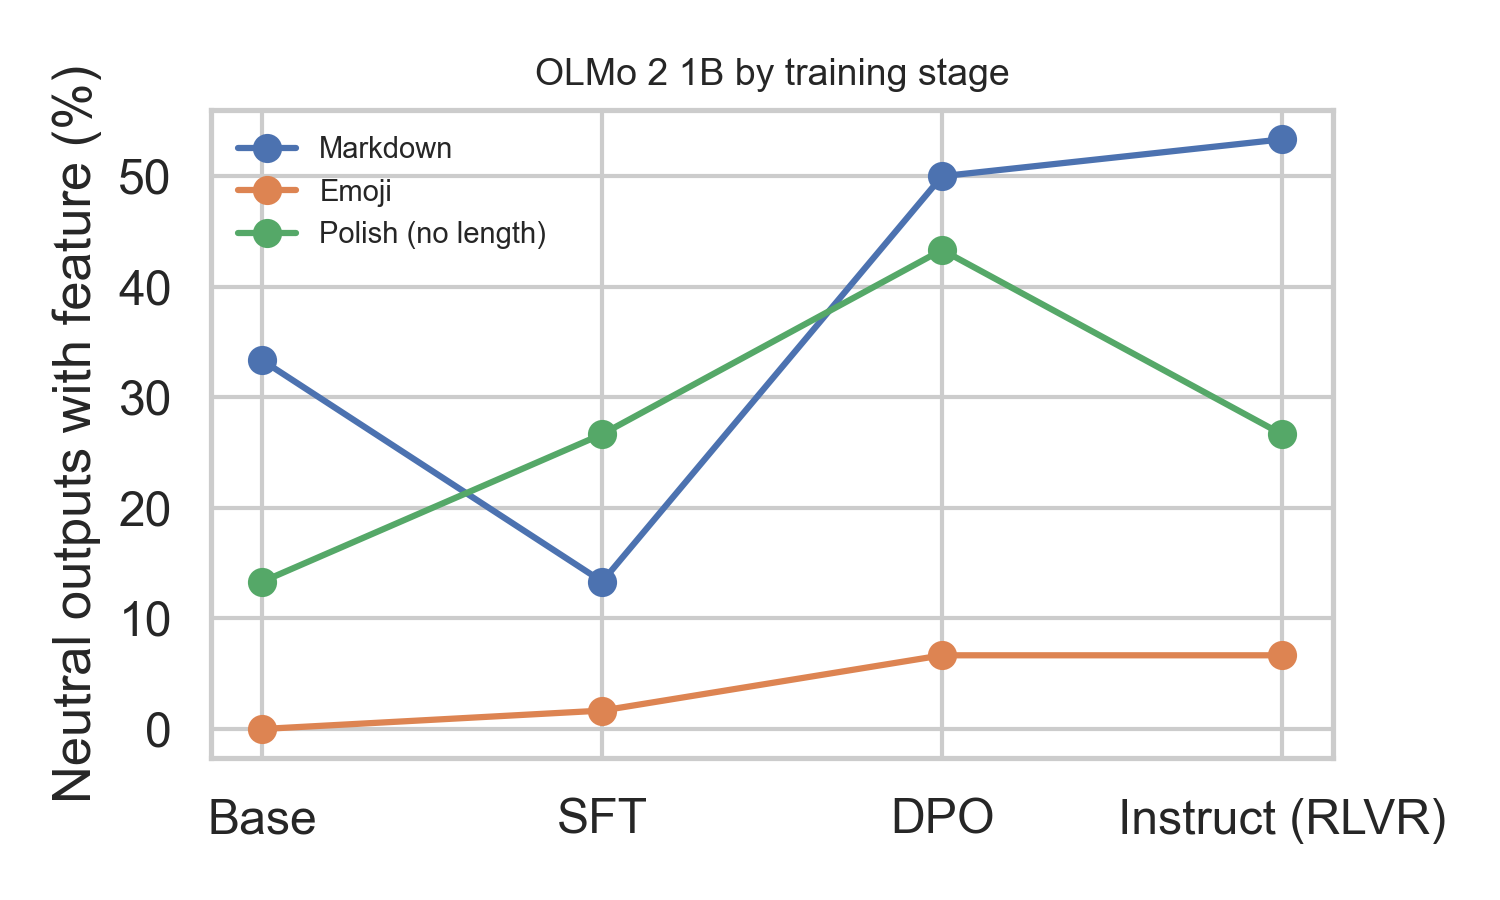
\includegraphics[width=0.6\linewidth]{../analysis_output/exp8_v2/olmo_stage_trend.png}
\caption{Neutral-condition feature rates across the OLMo 2 1B training stages (60 outputs per stage).}
\label{fig:olmo-stages}
\end{figure}

The Markdown default appears at the preference-optimization step. Paired over prompts, moving from the SFT to the DPO checkpoint raises the Markdown rate by 36.7 points (13.3\% to 50.0\%, $p=0.0002$) and Markdown density from 0.6 to 3.2 markers per 100 words ($p=0.0002$). Outputs also lengthen (75 to 189 words), but the density increase shows that the change is not only a length effect. The final RL stage changes neither rate (+3.3 points, $p=0.81$) nor density ($p=0.39$). Emoji stays rare at every stage (at most 6.7\%), and no stage-to-stage change in emoji is significant.

The ability to suppress Markdown on request appears at the same step. Relative to the placebo, the plain instruction has no detectable effect on the base ($+3.3$ points, $p=0.85$) or SFT checkpoint ($+11.7$, $p=0.09$), but it removes 45.0 points of Markdown at DPO and 65.0 points at the final stage (both $p=0.0002$). In this model family, preference optimization thus installs both the formatting default and the controllability that our other studies take for granted. The base checkpoint produces Markdown in 33.3\% of outputs, but it writes four times as many words as SFT (297 versus 75) and continues web-like text, so we do not interpret the base-to-SFT drop as removing a pretraining prior.

Two cautions apply. The evidence comes from one 1B model family, so it is consistent with, but does not establish, the account that preference data rewards formatted responses \cite{zhang2025lists}. And a placebo instruction \emph{raises} Markdown at the DPO and final stages (by 23.3 and 21.7 points), the opposite of the large hosted models in Study 4, so spillover direction depends on the model.

\section{Instruction Spillover}
\label{sec:spillover}

The placebo in Study 4 names no presentation feature, yet it removes emoji from every model that uses emoji: by 43.9 points (Qwen), 31.7 (Gemini), 17.8 (Sonnet), and 8.9 (Haiku), each significant at $p\le0.017$. Its effect on Markdown depends on the model. It removes 64.4 points for Qwen, 62.8 for Gemini, and 35.0 for Llama 3.3 70B, and it has no detectable effect for either Claude model or Llama 3.1 8B. The emoji-only prohibition shows the same pattern from another direction: it removes 40.0 to 49.4 points of Markdown for Gemini, Qwen, and both Llama models, although it never mentions Markdown. The first-pass pilot found the same no-emoji spillover across four other routes (Appendix~\ref{app:pilot}).

Measured against the placebo, the content-specific effect of the plain instruction ranges from 97.2 points (Sonnet) to 11.1 points (Llama 3.3 70B). For models with large generic effects, a condition-versus-neutral contrast therefore overstates what the plain instruction itself accomplishes: for Llama 3.3 70B, the total reduction in Markdown is 46.1 points, of which 35.0 are matched by the placebo.

The placebo also changes how much models write and think. It shortens Gemini outputs (133 to 86 words) and lengthens Llama 3.1 8B outputs (147 to 185 words), and it was the condition most likely to make Qwen spend more than 1,500 hidden reasoning tokens before answering. Emoji, and for some models Markdown, appear to belong to a casual default register that any constraining instruction moves away from, consistent with the topic conditioning in Study 1. Whatever the mechanism, intervention studies of model formatting should include an instruction-matched control.

\section{Measurement Validity and Limitations}
\label{sec:validity}

\paragraph{Detectors.} No detector has yet been validated against human annotation. Known weaknesses:
\begin{itemize}
  \item The Markdown detector fires on a single list line or backtick, so plain numbered structure, common in legal notices, counts as Markdown.
  \item The stock-phrase lexicon has ten hand-picked words and does not respond to conditions.
  \item The emoji pattern includes check marks and geometric symbols (Study 1 sensitivity above).
  \item Colors are read only from hexadecimal codes, and the purple hue window (270--330$^\circ$) is one of several defensible choices; the purple result does not depend on it.
\end{itemize}
A two-annotator validation on a stratified sample of at least 300 outputs, with per-detector precision, recall, and agreement, is the next step.

\paragraph{Models and coverage.} Studies 1--3 use older routes: one names a retired GPT-3.5 snapshot, and the free GLM route has since been withdrawn. Study 4 covers three frontier models but no OpenAI model, and each collection used a single temperature. Qwen 3.6 Flash's outputs in Study 4 were generated with different token budgets depending on whether a retry was needed.

\paragraph{Training stage.} Study 5 uses one 1B model family with one output per prompt and condition. Its base checkpoint is prompted without a chat template and writes much longer outputs, so base-versus-post-trained comparisons mix training stage with prompt format. Replicating the stage comparison on larger open checkpoints is the most important next step.

\paragraph{Baselines.} We have no reference distribution of human-written text or human-designed palettes for the same prompts. Such baselines are needed before claiming that a model is more homogeneous than people are, particularly for Study 2.

\paragraph{Design.} Study 3 has no unconstrained arm, and Studies 1 and 3 are censored for GLM. Study 4's prompts were written by the authors (five per family) and cover short workplace and consumer texts only.

\section{Discussion}

Four regularities hold across the studies. Presentation priors exist and depend on topic and model: social genres trigger emoji, advisory text triggers Markdown, and palettes default to a few blues. When the requirement is stated and enumerated, these priors are largely suppressed, wherever the instruction is placed. Instructions also act beyond their content: emoji and Markdown fall after instructions that do not mention them. And in the one model family whose training stages are public, the Markdown default and the ability to suppress it both appear at the preference-optimization step, which links presentation priors to the format-bias literature on reward models and judges \cite{zhang2025lists,li2024style}.

The practical implications are narrower than ``prompts are not enough''. For surface requirements that users actually state, prompting works most of the time, and a deterministic check catches the residue cheaply. The larger exposure is for users who never state a requirement. They receive the model's priors (Markdown in a plain-text field, emoji in a formal notice, a stock blue palette) without having chosen them. Studying whether people notice or accept these defaults requires human-subject work that this article does not attempt.

For evaluation practice, we recommend reporting three quantities separately: the default rate under a neutral prompt, the content-specific effect of an intervention measured against an instruction-matched control, and the residual violation rate after an explicit constraint. Benchmarks that report only the last quantity miss the first two.

\section{Conclusion}

Language models fill unspecified presentation choices with consistent, topic- and model-dependent defaults. These defaults are mostly suppressed once requirements are stated, but instructions also change features they never mention, unconstrained color suggestions converge on a few conventional blues, and in one open model family the Markdown default emerges with preference optimization. Separating default rates, content-specific intervention effects, and spillover gives a more accurate picture of model formatting behavior than pooled compliance rates do. Larger stage-wise replications, validated detectors, and human baselines are the next steps.

\section*{Ethics and Disclosure}

This work analyzes model outputs only and involves no human subjects. Generative AI tools were used as research assistance for code development, critique, and drafting; all reported numbers were recomputed from the artifact by the authors.

\section*{Artifact Availability}

An anonymized artifact accompanies the submission. It contains the collection scripts (including the local checkpoint collector), the input CSVs for every study, and two analysis scripts: \path{analyze_tist_revision.py} regenerates the Study 1--3 tables and figures, and \path{analyze_exp8_v2.py} regenerates the Study 4 and 5 tables, contrasts, and figure. The pilot tables are regenerated and hash-checked by the package verifier.

\bibliographystyle{ACM-Reference-Format}
\bibliography{haips2026_refs,tist2027_presentation_priors_refs}

\appendix

\section{First-Pass Pilot (Experiment 8 v1)}
\label{app:pilot}

Before Study 4, a first-pass probe crossed four instruction-tuned routes (Llama 3.3 70B, Llama 3.1 8B, Qwen 2.5 7B Instruct, and Qwen 3.6 Flash), twelve prompt families with one prompt each, and five conditions, with two repeats per cell; all 480 planned outputs were collected (Table~\ref{tab:exp8-completeness}). Its pooled rates appear in Table~\ref{tab:exp8-condition-summary}. The \texttt{polish\_default} column includes word count above the neutral median of each prompt family, so about half of neutral outputs fire on length by construction; Study 4 does not use it. In the pilot, the no-emoji condition reduced Markdown from 78.1\% to 27.1\% (paired, prompt-family-clustered reduction 0.510, $p=0.0005$), the first sign of the spillover analyzed in Section~\ref{sec:spillover}. Table~\ref{tab:exp8-stage-summary} groups the pilot routes by provider label; this is provenance metadata, not a training-stage contrast. Table~\ref{tab:exp8-ci-contrasts} reports Wilson intervals and unpaired contrasts that treat outputs as independent; they are descriptive only.

\begin{table}[t]
\centering
\caption{Experiment 8 first-pass completeness.}
\label{tab:exp8-completeness}
\begin{tabular}{lr}
\toprule
Artifact & Count \\
\midrule
Expected matrix rows & 480 \\
Observed expected rows & 480 \\
Missing expected rows & 0 \\
Errored rows after dedupe & 0 \\
Unexpected artifact IDs & 0 \\
\bottomrule
\end{tabular}
\end{table}


\begin{table}[t]
\centering
\caption{Experiment 8 condition summary across 480 clean outputs.}
\label{tab:exp8-condition-summary}
\begin{tabular}{lrrrrr}
\toprule
Condition & $n$ & Format default & Polish default & Emoji & Markdown \\
\midrule
\texttt{neutral} & 96 & 80.2\% & 72.9\% & 19.8\% & 78.1\% \\
\texttt{no\_emoji} & 96 & 27.1\% & 22.9\% & 0.0\% & 27.1\% \\
\texttt{plain\_no\_markdown} & 96 & 2.1\% & 25.0\% & 0.0\% & 2.1\% \\
\texttt{diverse\_domain\_specific} & 96 & 64.6\% & 74.0\% & 5.2\% & 61.5\% \\
\texttt{polished\_but\_plain} & 96 & 6.2\% & 45.8\% & 0.0\% & 6.2\% \\
\bottomrule
\end{tabular}
\end{table}


\begin{table}[t]
\centering
\caption{Experiment 8 route-label summary.}
\label{tab:exp8-stage-summary}
\begin{tabular}{lrrrrr}
\toprule
Route-stage label & $n$ & Format default & Polish default & Emoji & Markdown \\
\midrule
\texttt{chat\_or\_instruct} & 120 & 40.0\% & 35.8\% & 10.8\% & 40.0\% \\
\texttt{instruct\_candidate} & 360 & 34.7\% & 52.2\% & 3.1\% & 33.3\% \\
\bottomrule
\end{tabular}
\end{table}


\begin{table}[t]
\centering
\caption{Experiment 8 selected intervals and planned contrasts.}
\label{tab:exp8-ci-contrast}
\begin{tabular}{lrrrr}
\toprule
Condition/feature & Rate & 95\% CI & Delta vs. neutral & FDR q \\
\midrule
Neutral format default & 80.2\% & [71.1, 86.9]\% & -- & -- \\
Neutral Markdown & 78.1\% & [68.9, 85.2]\% & -- & -- \\
Neutral emoji & 19.8\% & [13.1, 28.9]\% & -- & -- \\
No-emoji emoji & 0.0\% & [0.0, 3.8]\% & -0.198 & $2.58\times10^{-6}$ \\
Plain-no-Markdown format default & 2.1\% & [0.6, 7.3]\% & -0.781 & $<10^{-12}$ \\
Plain-no-Markdown Markdown & 2.1\% & [0.6, 7.3]\% & -0.760 & $<10^{-12}$ \\
Polished-but-plain format default & 6.2\% & [2.9, 13.0]\% & -0.740 & $<10^{-12}$ \\
Polished-but-plain polish default & 45.8\% & [36.2, 55.8]\% & -0.271 & $3.63\times10^{-4}$ \\
\bottomrule
\end{tabular}
\end{table}


\end{document}
